\newpage
\chapter{Фрактальные $k$-кубы, являющиеся дендритами}

В этой главе рассматриваются фрактальные $k$-кубы --- многомерный аналог фрактальных квадратов.
Мы описываем последовательность действий, по которым можно определить, является ли данный фрактальный куб дендритом.

\begin{definition}
[Olsen L. (1998) \cite{Olsen1998}; Lau K., Luo J.J.,Rao H. (2013) \cite{LLR2013}]
Пусть  $D=\{d_1,\ldots,d_r\},\; d_i\in\{0,1,\ldots,n-1\}^k$, где $n\ge 2$, а $1<\#D<n^k$.\\
{\em Фрактальным $k$-кубом} порядка $n$ с {\em множеством единиц $D$} называют компактное множество $K\IN\rr^k$, удовлетворяющее $$K=\dfrac{K+D}{n}$$
\end{definition}

\begin{figure}[H]
    \centering
    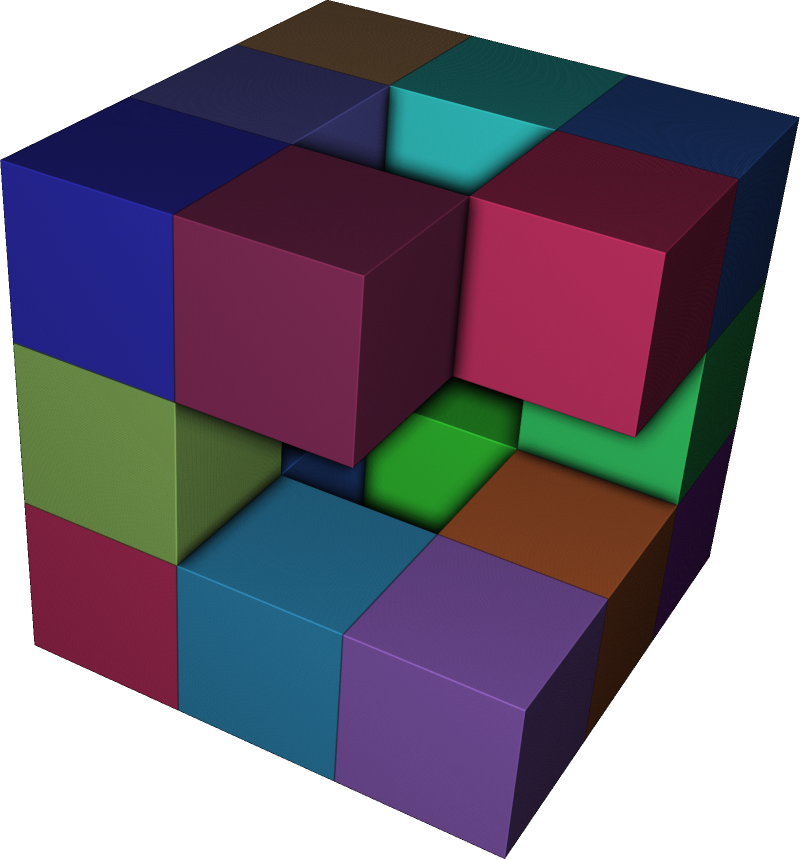
\includegraphics[width=0.45\textwidth]{FQD.png}
    \hfill
    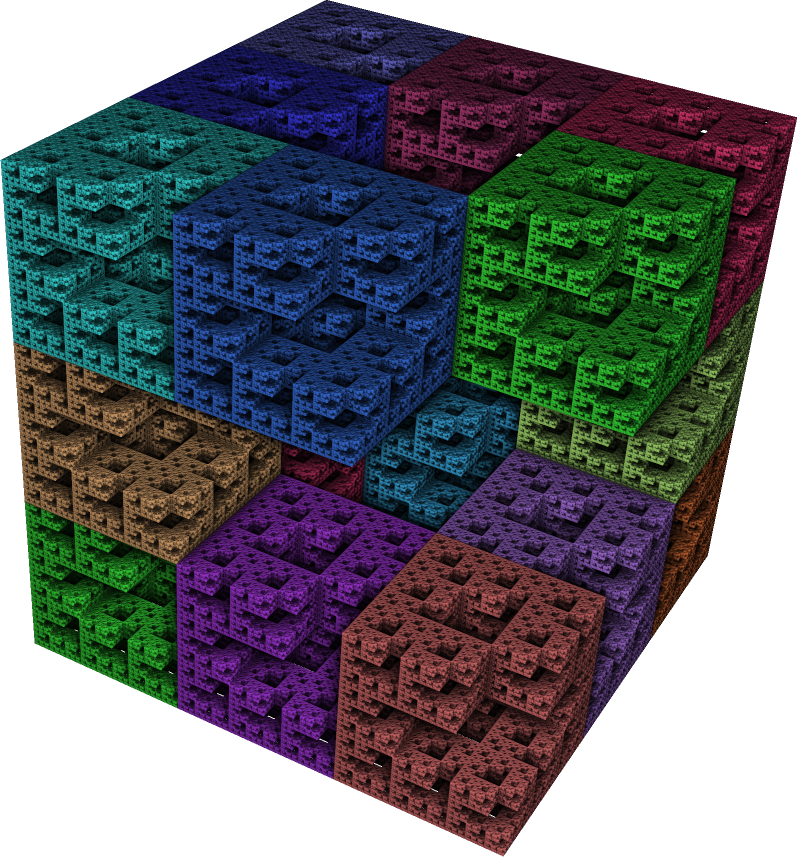
\includegraphics[width=0.45\textwidth]{FQK.png}
    \caption{Фрактальный куб}
    % \label{fig:enter-label}
\end{figure}

В случаях, когда $k=1$, $k=2$ и $k=3$, мы называем $K$  \emph{фрактальным отрезком}, \emph{фрактальным квадратом} и \emph{фрактальным кубом} сответственно.

\begin{remark}
Фрактальный $k$-куб $K=\dfrac{K+D}{n}$ с множеством единиц $D=\{0,1,\ldots,n-1\}^k$ есть единичный $k$-мерный куб $P^k=[0,1]^k$.
\end{remark}

Из этого можно сделать естественный вывод о том, что любой фрактальный $k$-куб $K$ содержится в единичном $k$-мерном кубе $P^k$ как его податтрактор.\\


Разобьём единичный $k$-куб $P^k$ на $n^k$ малых $k$-кубов $P^k_i$ с ребром $1/n$.
У каждого малого $k$-куба $P^k_i$ координата блидайшей к нулю вершины имеет вид $\frac{d_i}{n}$, где $d_i\in\{0,1,\ldots,n-1\}^k$.


Большенство определений, связанных с гранями единичного квадрата, фрактального квадрата и его самоподобной границей, естественным оброзом применяются и на фрактальные $k$ кубы, с поправкой на иную размерность.



\section{Грани $k$-куба $P^k$ и фрактального $k$-куба $K$} 
 
\subsection{Семейство граней единичного $k$-куба} 

Каждый фрактальный $k$-куб является подмножеством единичного $k$-куба $P^k$ в $\rr^k$, поэтому мы вводим некоторые обозначения, связанные с границей, гранями и сечениями единичного куба $P^k$.

Обозначим через $A_k$ множество $\{-1,0,1\}^k$. 
Существует естественное взаимно однозначное соответствие между семейством всех граней куба $P^k$ и множеством $A_k$.
Чтобы установить это, мы рассмотрим центр $(1/2,\ldots,1/2)$ куба $P^k$, который мы обозначим как $c$.
Каждому вектору $\bma=(\al_1,\ldots\al_k)\in A_k$ мы ставим в соответствие единственную грань $P_\bma$ куба $P^k$, центром которого является $c_\bma=c+\bma/2$, и наоборот. 
Противоположный вектор $-\bma$ определяет грань $P_{-\bma}$ с центром $c_{-\bma}=c-\bma/2$, которая параллельна и противоположна грани $P_{\bma}$, и следовательно, $P_{-\bma}+\bma=P_\bma$. 

 
\begin{figure}[H]
    \centering
    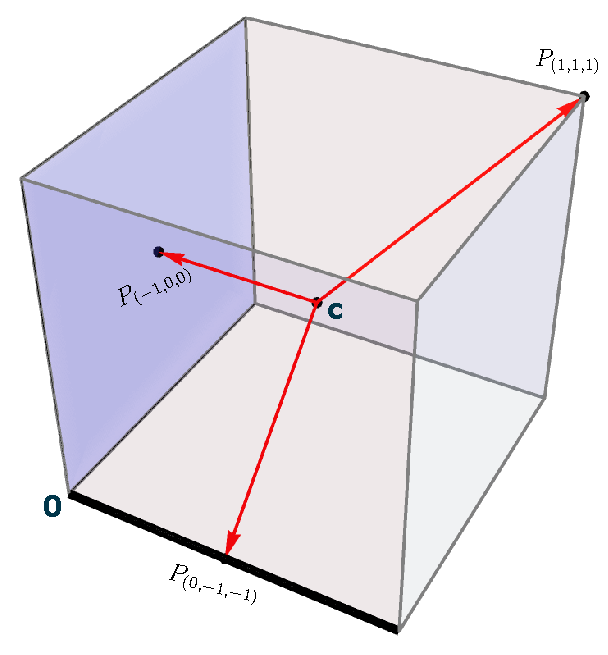
\includegraphics[width=0.55\textwidth]{faces.pdf}
    \caption{Грани $P_\bma$ единичного куба}
    \label{fig:uq_faces}
\end{figure}

Равенство $P_{-\bma}+\bma=P_\bma$ показывает, что кубы $P^k$ и $P^k+\bma$ пересекаются по своей общей грани. 
Эта общая грань является гранью $P_\bma$ куба $P^k$, и также гранью $P_{-\bma}+\bma$ куба $P^k +\bma$.\\

Для элементов из $A_k$ существует отношение порядка $\sqsubseteq$ на $A$, равносильное отношению включения $\supseteq$ граней куба $P$ и аналогичное отношению из Определения \ref{Aorder}.
Пусть $\bma=(\al_1,\al_2,\ldots,\al_k)\in A_k$, $\bmb=(\be_1,\be_2,\ldots,\be_k)\in A_k$.
Будем говорить, что $\bma\sqsubseteq\bmb$, если из $\al_i\neq 0$ следует $\be_i=\al_i$.
Другими словами, отношение $\bma\sqsubseteq\bmb$ равносильно включению $P_\bma\supseteq P_\bmb$
Если при этом $\bma\neq\bmb$, то $\bma\sqsubset\bmb$.\\

Поскольку $P_\bma=P^k\cap(\bma+P^k)$, то множество
$\{\bma+P^k, \bma\in A\mmm \{0\}\}$ --- это множество всех соседей $P ^ k$ в семействе $\{d+P^k, d\in\zz^k\}$, а граница $P^k$ представлена формулой 
\begin{equation}\label{dpk}
\dd P^k=\bigcup\limits_{\bma\in A_k\mmm \{0\}}P_\bma
\end{equation}

{\bf ДОБАВИТЬ ГРАНИ ФРАКТАЛЬНОГО КУБА\\
И ПЕРЕПИСАТЬ СЛЕДУЮЩИЙ РАЗДЕЛ}

\begin{definition} 
Пусть $K$ --- фрактальный $k$-куб.
Для $\bma\in A_k\mmm\{0\}$ обозначим множество $K_\bma:=K\cap P_\bma$ и назовём его $\bma$-гранью фрактального $k$-куба $K$.
\end{definition}

\begin{theorem}\label{bma0}
Для каждого $\bma\in A_k$ соответсвующая ему грань $K_\bma = K\cap P_\bma$ является фрактальным $k$-кубом с множеством единиц $D_\bma = D\cap(n-1)P_\bma$.
\end{theorem}

\begin{figure}[H]
\centering
\includegraphics[width=0.4\textwidth]{images/presentation/Qk.png}
\hfill
\includegraphics[width=0.4\textwidth]{images/presentation/Qk_a.png}
\caption{Фрактальный куб и его двумерная грань}
\end{figure}


\section{Пересечение фрактальных кубов}

Пусть $K_1, K_2$ --- фрактальные $k$-кубы порядка $n$ с множествами единиц $D_1, D_2$ и обозначим $F_0=K_1\cap K_2$.

Чтобы понять структуру множества $F_0$, нам нужно принять во внимание все возможные пересечения $F_\bma=K_1\cap (K_2+\bma)$,
где $\bma\in A_k$ и установить отношения между всеми этими множествами.

\subsection{Множества $F_\al$ и связанные с ними множества единиц}

$\bma$- и $(-\bma)$-грани фрактальных кубов $K_1$ и $K_2$ равны $K_{1,\bma}=K_1\cap P_\bma$ и $K_{2,-\bma}=K_2\cap P_{-\bma}$ соответственно.
Следовательно, $F_\bma$ может быть представлено как пересечение $K_{1,\bma}\cap (K_{2,-\bma}+\bma)$.

Множество единиц для $K_{1,\bma}$ --- это $D_{1,\bma}= D_1\cap(n-1)P_\bma$, а множество единиц для $K_{2,-\bma}$, соответственно, есть ни что иное как $D_{2,-\bma}= D_2\cap(n-1)P_{-\bma}$.
Следовательно, фрактальный куб $(K_{2,-\bma}+\bma)$ имеет множество единиц $D_2\cap(n-1)P_{-\bma}+(n-1)\bma$.
   
\begin{proposition}\label{falfa}
Пусть $K_1,K_2$ --- фрактальные $k$-кубы порядка $n$ с множествами единиц $D_1, D_2$ и пусть $\bma\in A_k$.
Множество $F_\bma$ является пересечением фрактальных кубов $\hat K_1,\hat K_2$, множества единиц которых равны $\hat D_1=D_1\cap(n-1)P_\bma$ и $\hat D_{2}=D_2\cap(n-1)P_{-\bma}+(n-1)\bma$ соответственно.

Более того, для любого $\bmg\perp\bma$ множество $F_{\bma+\bmg}$ является пересечением $\hat K_{1}\cap(\hat K_{2}+\bmg)$.
\end{proposition}  

\begin{proof} 
Первое утверждение уже было доказано выше. Давайте проверим второе.

Если $\bmb=\bma+\bmg $, то $\bmb\sqsupset\bma$.
Множество $F_\bmb$ является пересечением фрактальных кубов с множествами единиц $D_{1,\bmb}=D_1\cap(n-1)P_\bmb$ и $D_{2,-\bmb}=D_2\cap(n-1)P_{-\bmb}+(n-1)\bmb$.
Поскольку $\bmb=\bma+\bmg$ and $P_\bmb=P_\bma\cap P_\bmg$, то мы получаем $D_{1,\bmb}=\hat D_{1}\cap(n-1)P_\bmg$ и $D_{2,\bmb}=\hat D_{2}\cap(n-1)P_{-\bmg}+(n-1)\bmg$.
\end{proof}


\begin{remark}\label{galfa}  
Второе утверждение Предложения \ref{falfa} показывает, что пересечение фрактальных кубов $\hat K_1$ и $\hat K_2$ и всех их граней также может рассматриваться независимо от исходных множеств $K_1, K_2$.\\
Пересечение $G_\bma$ множеств единиц $D_1\cap(n-1)P_\bma$ и $D_2\cap(n-1)P_{-\bma}+(n-1)\bma$ равно $G_\bma=D_1\cap(D_2+(n-1)\bma)$ и естественным образом связано с множеством $F_\bma$.
Если $\bma=0$, то множество $G_\bma$ имеет вид $G_0=D_1\cap D_2$.
\end{remark}
 
\begin{remark}\label{qbma}
Обозначим  фрактальный куб с набором цифр $G_\bma$ как $Q_\bma$.
Он удовлетворяет выражению $Q_\bma=\frac{1}{n}(Q_\bma+G_\bma)$, а значит $\dim_H(Q_\bma)=\log_n\#G_\bma$.
\end{remark} 
  
  
\subsection{Теорема о пересечении фрактальных кубов}
 
Следующая теорема устанавливает отношения между множествами $F_\bma$:

 
\begin{theorem}\label{IFC}
Семейство $\{F_\bma, \bma\in A_k\}$ пересечений $F_\bma =K_{1}\cap (K_{2}+\bma)$ удовлетворяет системе $\Sa$ уравнеий
 
\begin{equation}\label{perall}
F_\bma=\bigcup\limits_{\bmb\sqsupseteq{\bma}}T_{\bma\bmb}(F_\bmb),\qquad \bma\in A_k,
\end{equation}
 
где для каждого $\bmb\sqsupseteq\bma$, 
\begin{equation}\label{Gab}
T_{\bma\bmb}(F_\bmb)=\frac{1}{n}(F_\bmb+G_{\bma\bmb})\mbox{\quad  \text{и} \quad}
  G_{\bma\bmb}=D_1\cap(D_2+n\bma-\bmb)
\end{equation}
\end{theorem}

 

\begin{proof}
Представим $F_\bma$ как $K_1\cap (K_2+\bma)=\dfrac{1}{n}\bigl((K_1+D_1)\cap (K_2+D_2+n\bma)\bigr).$ \\

Пусть $d_1\in D_1$ и $d_2\in D_2$, тогда пересечение $(K_{1}+d_1)\cap (K_{2}+d_2+n\bma)$ непусто если $(P+d_1)\cap (P+d_2+n\bma)\neq\0$, что означает, что вектор $\bmb=d_2-d_1+n\bma$ лежит в множестве $A$. 
Поскольку для любого номера координаты $i=1,\ldots  ,k$ мы имеем $|(d_2-d_1)_i|\le n-1$, это возможно только если $\bmb\sqsupseteq \bma$.\\

Если $\bmb=\bma$, то $d_1=d_2+(n-1)\bma$, следовательно $d_1\in D_1\cap(D_2+(n-1)\bma)= G_\bma$.

Если $\bmb\sqsupset\bma$, то $(K_{1}+d_1)\cap (K_{2}+d_2+n\bma)=(K_1\cap (K_2+\bmb))+d_1$, и $d_1\in D_1\cap(D_2+n\bma-\bmb)$. Множество $D_1\cap(D_2+n\bma-\bmb)$ мы обозначим как  $G_{\bma\bmb}$. 

Заметим, что  $G_{\bma\bma}=D_1\cap(D_2+n\bma-\bma)$, а значит $G_{\bma\bma}=G_{\bma}$.

В результате мы получаем  $F_\bma=\frac{1}{n}\bigcup\limits_{\bmb\sqsupseteq{\bma}}(F_\bmb+G_{\bma\bmb})=
\frac{1}{n}(F_\bma+G_\bma)\cup\bigcup\limits_{\bmb\sqsupset{\bma}}\frac{1}{n}(F_\bmb+G_{\bma\bmb})$.
\end{proof}\bigskip

Отношения между множествами $F_\bma$, установленные в Теореме \ref{IFC} приводят к {\em структурному графу $\Ga_\Sa$} системы $\Sa$, определенной в \eqref{perall}. 
С помощью этой систему и графа можно найти важные свойства множеств $F_\bma$.

\begin{definition}
Структурный граф $\Ga_\Sa$ является ориентированным графом, в котором все вершины являются непустыми множествами $F_\bma$ и для каждого $\bma\sqsubseteq\bmb$ существует ребро $(F_\bma,F_\bmb)$, направленное из $F_\bma$ в $F_\bmb$ и соответствует оператору $T_{\bma\bmb}$, если этот оператор невырожденный.
\end{definition}

В общем случае граф $\Ga_\Sa$ будет содержать $3^k$ вершин и $5^k$ ребер, и $3^k$ из этих ребер являются циклами от $F_\bma$ к самому себе.
Мы помечаем каждое ребро символом $G_{\bma\bmb}$.\\

Тем не менее, некоторые вершины и ребра в графе $\Ga_\Sa$ могут исчезнуть.
Это происходит для тех $F_\bma$, которые пусты, и для тех ребер $(F_\bma,F_\bmb)$, для которых $T_{\bma\bmb}(F_\bmb)=\0$, то есть 
\begin{equation}\label{Tempty}
T_{\bma\bmb}(F_\bmb)=\0\mbox{\quad   \text{если}  \quad  }G_{\bma\bmb}=\0\mbox{ \quad   \text{или} \quad   }F_\bmb=\0.
\end{equation} 

Множество $F_\bma$ пусто, если $G_\bma=\0$ и для любого $\bmb\sqsupset\bma$ множество $F_\bmb+G_{\bma\bmb}=\0$. 
Применяя \eqref{Tempty} ко всем $\bmb\sqsupset\bma$, мы выводим следующее условие пустоты для $F_\bma$:

\begin{lemma}
Множество $F_\bma=\0$ тогда и только тогда, когда для любого $\bmb\sqsupseteq\bma$ и для любой конечной последовательности\\ $\bma=\bma_0\sqsubseteq\bma_1\sqsubseteq\ldots \bma_{p-1}\sqsubseteq\bma_p=\bmb$ произведение 
$\#G_{\bma_0\bma_1}\#G_{\bma_1\bma_2}\ldots  \#G_{\bma_{p-1}\bma_p}\#G_{\bmb}$ равно нулю. 
\qed
\end{lemma}


По этим причинам, из-за сокращения всех пустых вершин и ребер, структурный граф $\Ga$ для системы $\Sa$, определенный в теореме \ref{IFC}, имеет множество вершин $V_\Sa=\{F_\bma: \bma\in A, F_\bma\neq\0\}$ и множество ребер
$E_\Sa=\{(F_\bma, F_\bmb): \bma\sqsubseteq\bmb, G_{\bma\bmb}\neq\0, F_\bmb\neq\0\}$. 

Вообще такой граф $\Ga_\Sa$ может быть и несвязен.

\begin{definition}
Мы говорим, что пара вершин $F_\bma, F_\bmb, \bma\sqsubset\bmb$ {\em соединена направленным путем} в графе $\Ga_\Sa$, если существует конечная последовательность  $\bma=\bma_0\sqsubset\bma_1\sqsubset\ldots \bma_{p-1}\sqsubset\bma_p=\bmb$ такая, что для любых  $j=0,\ldots  ,p$ множества $F_{\bma_j}\neq\0$  и множества $G_{\bma_{j-1}\bma_j}\neq\0$ для $j=1,\ldots  ,p$.   
\end{definition}

Мы пишем $\bmb\succ\bma$, если в $\Ga$ есть направленный путь от $F_\bma$ до $F_\bmb$.

Если $\bmb\succcurlyeq\bma$ или $\bma\succcurlyeq\bmb$, то мы говорим, что $\bma$ и $\bmb$ являются $\Ga${\em-сравнимы}.

Мы обозначим через $\Ga_\bma$ подграф в $\Ga$, все вершины которого являются $F_\bmb$ такими, что $\bmb\succcurlyeq\bma$. 
Мы говорим, что $\bmb$ является {\em максимальным} для $\Ga_\bma$, если $\Ga_\bmb$ является единственной вершиной $F_\bmb$.
Мы говорим, что $\bmb$ является {\em минимальным} для $\Ga_\Sa$, если нет $\bma$ такого, что $\bma\prec\bmb$.

Стоит отметить, что, согласно предложению \ref{falfa}, граф $\Ga_\bma$ показывает множество всех уравнений, которые полностью определяют каждое из множеств $F_\bmb$, для которых $\bmb\succcurlyeq\bma$.\\

Каждый оператор $T_{\bma\bmb}$, соответствующий некоторому ребру в графе $\Ga_\Sa$, является непустым конечным объединением гомотетий, поэтому он сохраняет размерность, т.е. для любого подмножества $X\IN F_\bmb$, $\dim_H(T_{\bma\bmb}(X))=\dim_H(X)$.\\


\begin{example} 
[Пересечение двух фрактальных квадратов, состоящее из $24$ точек, и его стркутурный граф $\Ga_\Sa$.]

Рассмотрим пересечение фрактальных квадратов $K_1$ и $K_2$ порядка $6$ с множествами единиц $D_1$ и $D_2$.
На рисунке слева ниже мы представляем множества единиц множеством красных клеток $T_1(P)=\dfrac{D_1+P}{6}$ и синих клеток $T_2(P)=\dfrac{D_2+P}{6}$ .
Справа видны фрактальные квадраты $K_1$ и $K_2$. \\

Большинство из множеств $G_\bma$, а именно, \\
$G_0,G_{(1,0)},G_{(-1,0)},G_{(0,1)},G_{(0,-1)},G_{(1,1)},G_{(1,-1)},G_{(-1,1)}$ являются пустыми, и только $G_{(-1,-1)}=(0,0)$. Следовательно, 
$F_{(1,1)}=F_{(1,-1)}=F_{(-1,1)}=\0$ и $F_{(-1,-1)}=\{(0,0)\}$.\\


\begin{figure}[H]
    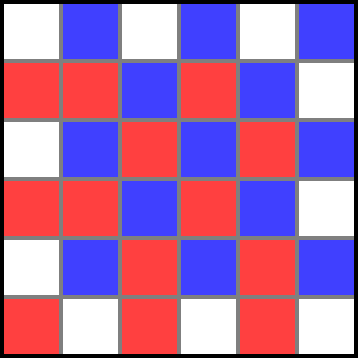
\includegraphics[width=0.45\textwidth]{FSI_6x6_DS.pdf}
    \hfill
    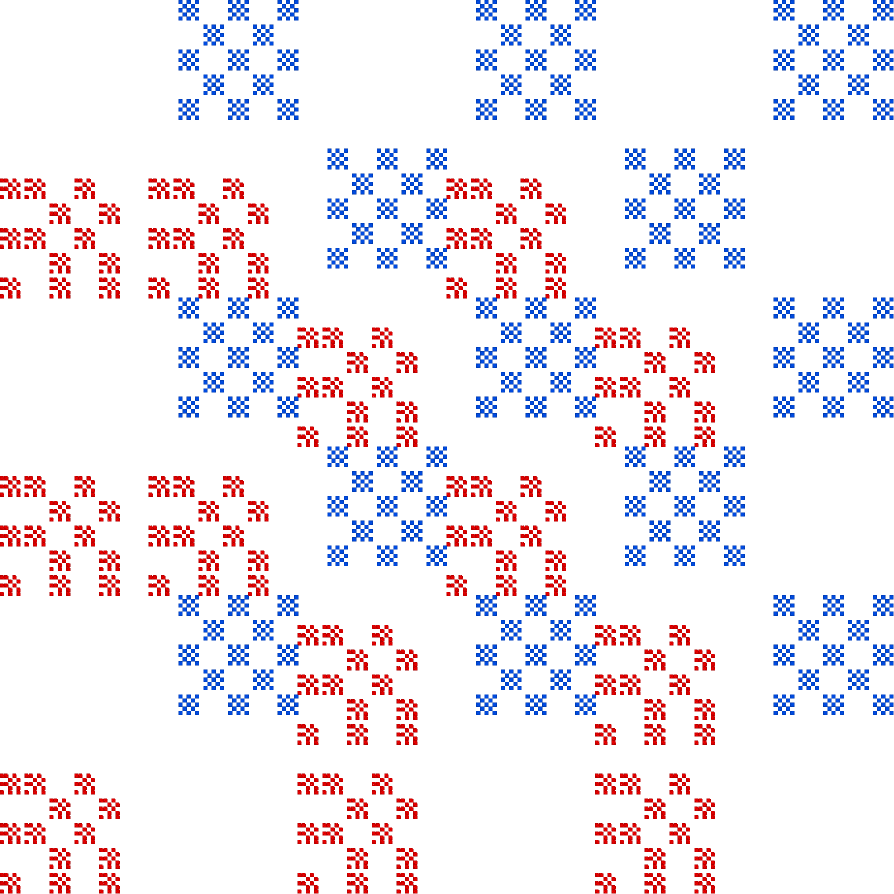
\includegraphics[width=0.45\textwidth]{FSI_6x6_K.png}
    \caption{Диаграмма множеств единиц для $D_1$ и $D_2$ (слева) и фрактальные квадраты $K_1$ и $K_2$ (справа).}
    % \label{fig:my_label}
\end{figure}


Множество $F_{(1,0)}$ пусто, поскольку $G_{(1,0)},F_{(1,1)}$ и $F_{(1,-1)}$ пусты. 
По той же причине $F_{(0,1)}=\0$. \\

Множества $G_{(-1,0)(-1,-1)}=\{(0,2),(0,4)\}$ и \\
$G_{0(-1,0)}=\{(1,2),(1,4),(2,3),(3,2),(3,4),(4,3)\}$.
Множества $G_{(0,-1)(-1,-1)}$ и $G_{0(0,-1)}$ получены их предыдущих двух.\\

Таким образом, после удаления пустых вершин и ребер
граф $\Ga_\Sa$ содержит четыре вершины  $F_0,F_{(-1,0)},F_{(0,-1)},F_{(-1,-1)}$ и четыре ребра, которым соответствуют $G_{(-1,0)(-1,-1)}, G_{(0,-1)(-1,-1)},G_{0(-1,0)}$ и $G_{0(0,-1)}$.

Вычисление с использованием формулы \eqref{perall} показывает, что
$\#F_{(-1,0)}=\#F_{(0,-1)}=2$ и $\#F_0=2 \#G_{0(-1,0)}+2\#G_{0(0,-1)}=24.$


\begin{figure}[H]
    \centering
    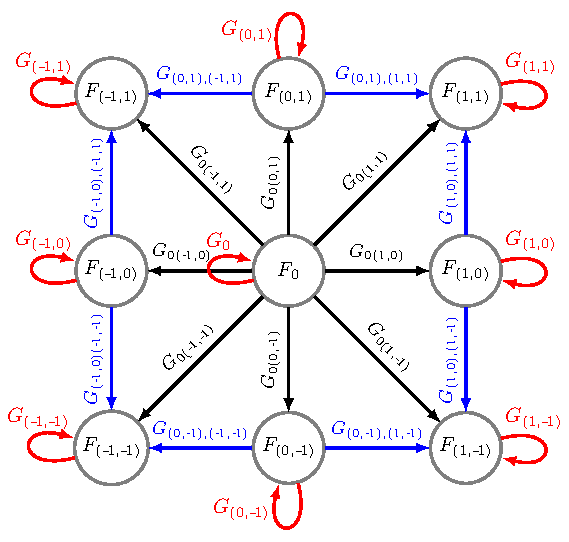
\includegraphics[width=.5\textwidth]{structure_grapg_full.pdf}
    \hfill
    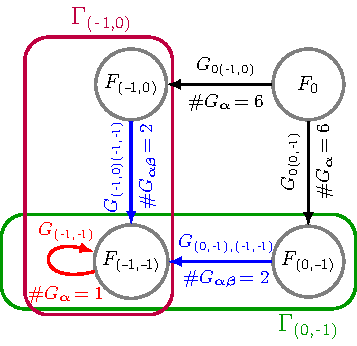
\includegraphics[width=.45\textwidth]{FSI_6x6_SG.pdf}
    \caption{Структурный граф $\Ga_\Sa$ в общем случае для пересечения двух фрактальных квадратов (слева) и сокращённый граф $\Ga_\Sa$ для Примера 1 (справа). На рисунке справа выделены подграфы $\Ga_{(-1,0)}$ и $\Ga_{(0,-1)}$. }
\end{figure} 
\end{example} 


\subsection{Мощность множества $F_\al$.}

\begin{theorem}\qquad
\begin{enumerate}[nolistsep]
\item Множество $F_\bma$ является одноточечным, если $\Gamma_\bma$ представляет собой цепочку $\bma=\bma_1\prec\ldots\prec\bma_p$, в которой для всех $j\le p-1$, $\# G_{\bma_j\bma_{j+1}}=1$, $G_{\bma_j}=\0$ и $\#G_{\bma_p}=1$;
\item Множество $F_\bma$ конечно, если для всех максимальных вершин $\bmb$ в $\Gamma_\bma$, верно $\#G_\bmb=1$ и $G_{\bmb}=\0$ для всех остальных вершин в $\Gamma_\bma$.
В этом случае $\#F_\bma$ равно сумме всех композиций $\prod \limits_{j=1}^{p-1}\# G_{\bma_j\bma_{j+1}}$, взятых по всем цепочкам $\bma=\bma_1\prec\ldots\prec\bma_p=\bmb$, где $\bmb$ является максимальным в $\Gamma_\bma$;
\item Множество $F_\bma$ счетно, если $\#G_\bmb\le 1$ для всех вершин $\bmb$ в $\Gamma_\bma$;
\item Множество $F_\bma$ несчетно, если в $\Gamma_\bma$ существует такая вершина $\bmb$, что $\#G_\bmb> 1$.
\end{enumerate}
\end{theorem}

\begin{corollary}
Фрактальный куб $K$ обладает свойством одноточечного пересечения, если структурный граф $\Gamma(\Sa)$ представляет собой объединение цепочек $0\prec\bma_{i1}\prec\ldots\prec\bma_{ip_i}$, для которых все $\bma_{ij}$ различны и таковы, что для всех $i$ верно $\#G_{\bma_{ip_i}}=1$ и для всех $i,j$ таких, что $j\le p_i-1$, верно $\# G_{\bma_{ij}\bma_{i,j+1}}=1$ и $G_{\bma_{ij}}=\0$.

Фрактальный куб $K$ обладает свойством конечного пересечения, если для всех максимальных $\bma$ в графе $\Ga (\Sa)$, $\#G_\bma=1$ и для всех остальных $\bma\neq 0$, $\#G_\bma=0$.
\end{corollary}

\begin{example}[Фрактальный куб с одноточечным пересечением]
Возьмем фрактальный куб $K=\dfrac{K+D}{4}$ с множеством единиц 
\begin{equation*}
\begin{split}
D=\{
    &(0,0,0), (1,1,1), (2,2,2), (3,3,3), (2,1,1), (1,2,1), (1,1,2), (1,2,2),\\ 
    &(2,2,1), (2,1,2), (0,0,2), (0,2,1), (3,3,1), (3,1,1), (2,0,0), (1,2,0),\\ 
    &(1,3,3), (1,1,3)\}     
\end{split}
\end{equation*}
 
\begin{figure}[H]
    \centering
    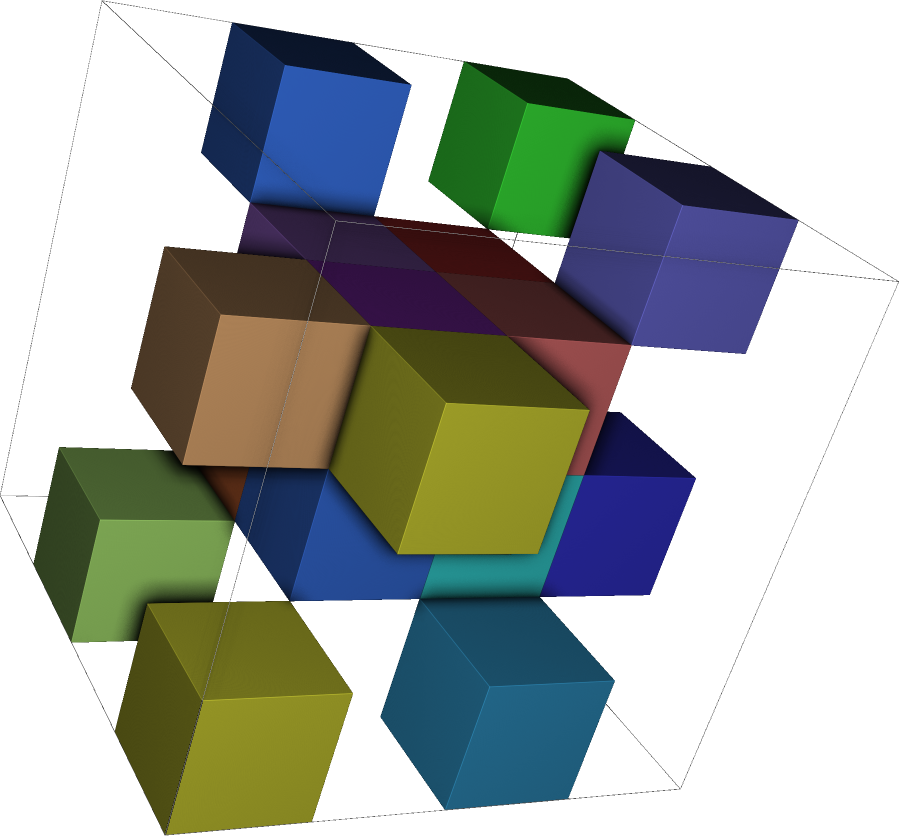
\includegraphics[width=0.45\textwidth]{fqP1a.png}
    \hfill
    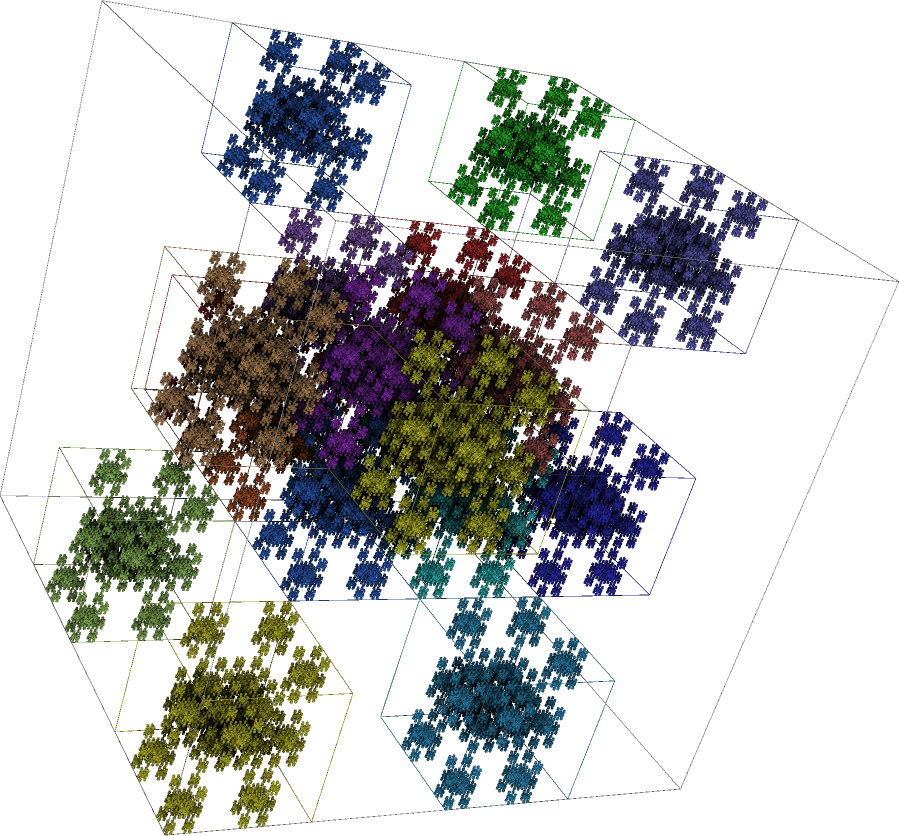
\includegraphics[width=0.45\textwidth]{fqK1a.png}
    \caption{Фрактальный куб с одноточечным пересечением}
    \label{fig:fq}
\end{figure}

\begin{figure}[H]
    \centering
    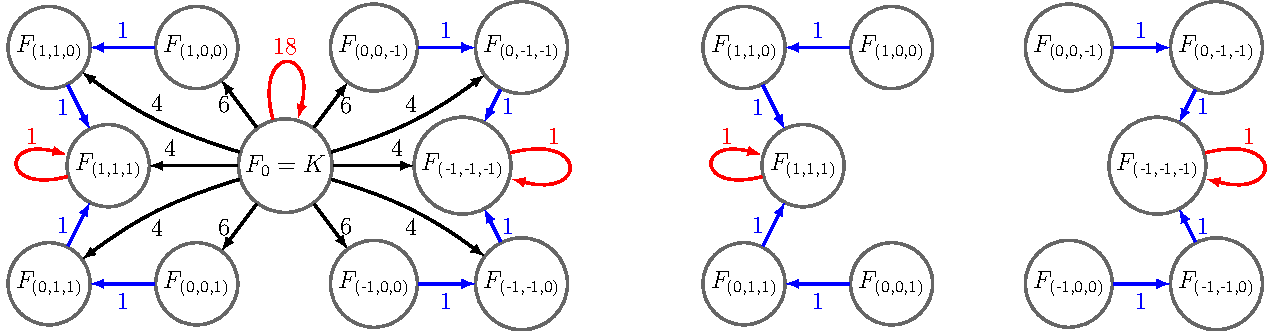
\includegraphics[width=\textwidth]{SG_for_FQ.pdf}
    \caption{Структурный граф}
    \label{fig:fq_sg}
\end{figure}
\end{example}

\begin{figure}[H]
    \centering
    \hfill
    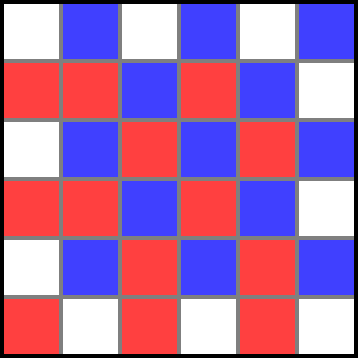
\includegraphics[width=0.45\textwidth]{FSI_6x6_DS.pdf}
    \hfill
    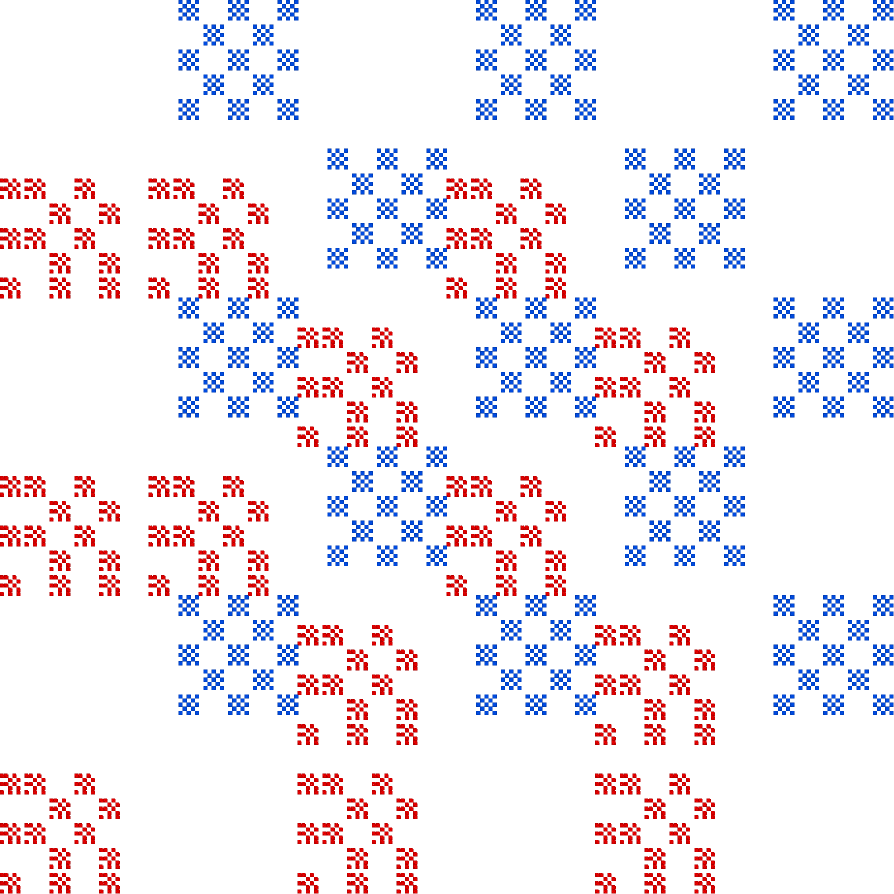
\includegraphics[width=0.45\textwidth]{FSI_6x6_K.png}
    \hfill
    \caption{Пересечение фрактальных квадратов по 24 точкам}
    \label{fig:FSI_6x6}
\end{figure}

\begin{example}[Пересечение по 24 точкам]
\label{ex:FSI_6x6}
На Рисунке \ref{fig:FSI_6x6} представлено пересечение двух фрактальных квадратов $K_1$ и $K_2$ порядка $6$ (синее и красное множество), а на Рисунке \ref{fig:FSI_SG} слева показан структурный граф $\Gamma_{\Sigma(K_1,K_2)}$ этого пересечения.
По этому графу легко понять, что пересечение $F_0$ конечно, причем $\#F_0=24.$
\end{example}

\begin{figure}[H]
    \centering
    \hfill
    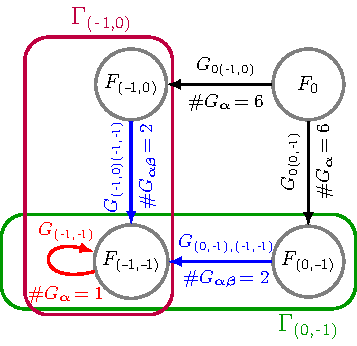
\includegraphics[width=0.35\textwidth]{FSI_6x6_SG.pdf}
    \hfill
    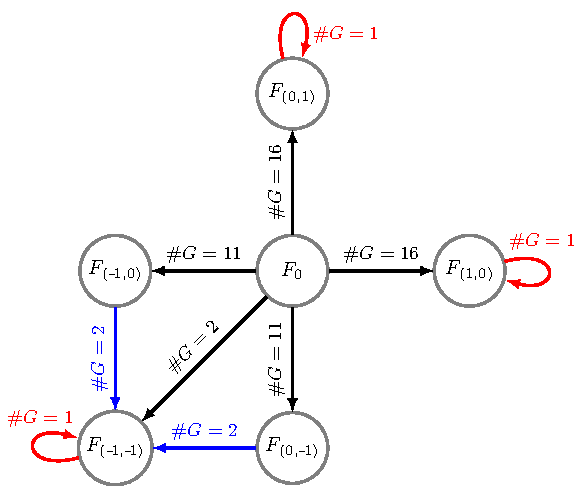
\includegraphics[width=0.55\textwidth]{FSI_7x7_SG.pdf}
    \hfill
    \caption{Структурные графы пересечений на рисунках \ref{fig:FSI_6x6} и \ref{fig:FSI_7x7}}
    \label{fig:FSI_SG}
\end{figure}

\begin{example}[Пересечение по 78 точкам]
\label{ex:FSI_6x6}
На Рисунке \ref{fig:FSI_7x7} представлено пересечение двух фрактальных квадратов $K_1$ и $K_2$ порядка $7$ (синее и красное множество), а на Рисунке \ref{fig:FSI_SG} справа показан структурный граф $\Gamma_{\Sigma(K_1,K_2)}$ этого пересечения.
По этому графу,аналогично предыдущему примеру, легко понять, что $\#F_0=78.$

\end{example}

\begin{figure}[H]
    \centering
    \hfill
    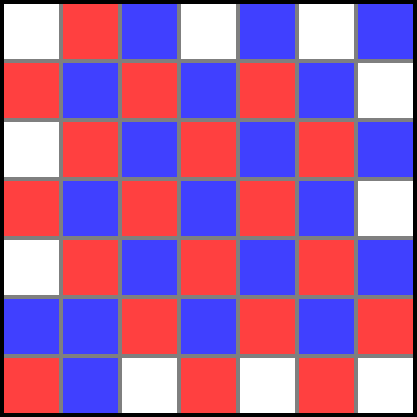
\includegraphics[width=0.45\textwidth]{FSI_7x7_DS.pdf}
    \hfill
    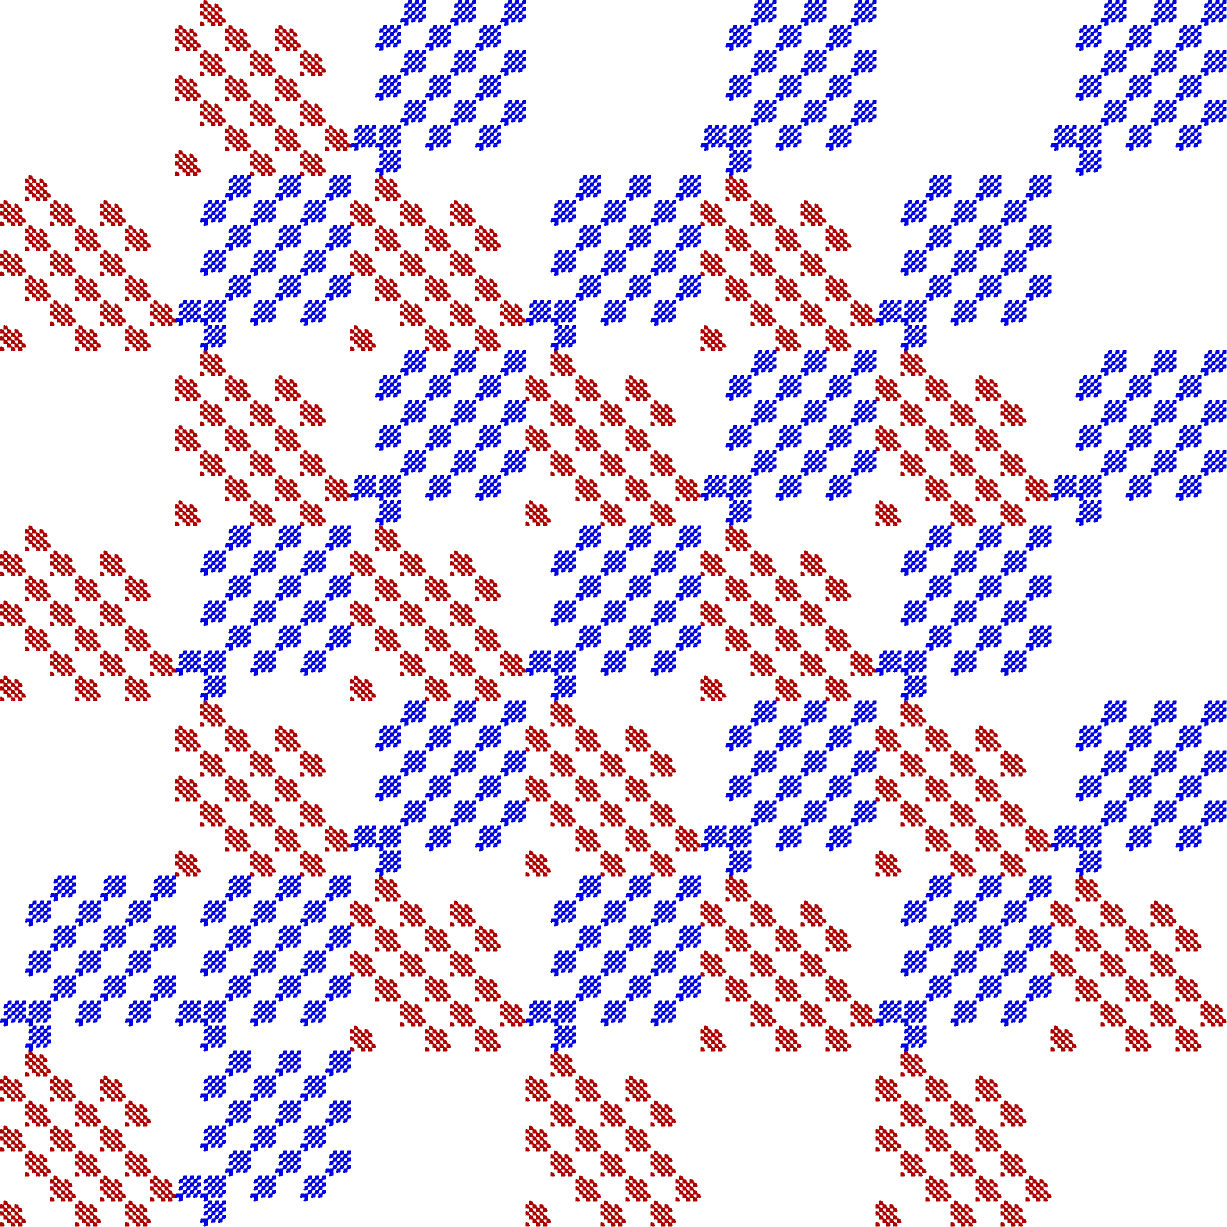
\includegraphics[width=0.45\textwidth]{FSI_7x7_K.png}
    \hfill
    \caption{Пересечение фрактальных квадратов по 78 точкам}
    \label{fig:FSI_7x7}
\end{figure}


\section{Дендритность фрактального куба}

В этом параграфе рассмотрим фрактальные кубы (с одноточечным пересечением) и проверим, является ли рассматриваемое множество дендритом.
Метод определения свойства дендритности фрактального куба основан на нахождении двудольного графа пересечений фрактального куба.

\subsection{Свойство одноточечного пересечения и критерий дендритности}

\begin{definition}\label{fipss}\cite{FIP}
Система множеств с одноточечным пересечением (было в главе 1)  
\end{definition}

\begin{definition}\label{fipcs}
Система сжимающих подобий со свойством одноточечного пересечения.(было в главе 1)
\end{definition}

\subsection{Алгоритм проверки фрактального куба на свойство дендритности}

Пусть $K$ --- фрактальный $k$-куб.
Чтобы проверить $K$ на наличие дендритности, нужно выполнить следующие шаги:

 \begin{enumerate}

    \item Найдём все множества $G_\bma, G_{\bma\bmb}$ для системы $\Sigma=\Sigma(K,K)$ и запишем систему $\Sa$.
    Согласно Определению \ref{strg} и Лемме \ref{red}, исключим все исчезающие вершины и ребра и построим граф $\Ga_\Sa$.
   
    \item Используя Следствие \ref{SIPQ}, проверим выполнение свойства одноточечного пересечения для $K$.
    Если это не удается, то $K$ не является дендритом.
    
    \item Построим двудольный граф пересечений для фрактального куба $K$, соединив рёбрами пересекающиеся копии с точкой пересечения этих копий. 
    Нужно учесть случай с кратными точками, упомянутыми в следствии \ref{mpoint}.
    Теперь если получившийся двудольный граф пересечений будет деревом, то $K$ --- дендрит.
    
\end{enumerate}